\documentclass[10pt, compress]{beamer}

\usetheme{m}

\usepackage{booktabs}
\usepackage{minted}

\usemintedstyle{trac}

\title{Worksheet 3: MPI Point-to-Point and One-Sided Communication}
\subtitle{Programming of Supercomputers [IN2190]}
\date{December 23, 2015}
\author{Group 09: Gerasimos Chourdakis, Nathaniel Knapp, Walter Simson}
\institute[TUM Informatics]{Fakult\"at f\"ur Informatik - Technische Universit\"at M\"unchen}

\begin{document}

\maketitle

\begin{frame}[fragile]{Agenda}
    \tableofcontents
\end{frame}


\section{Task 3: Base case}
\begin{frame}
  \frametitle{Cannon's algorithm}
  \begin{itemize}
  \item Parallel algorithm for multiplying 2D matrices.
  \item Suiable for $N \times N$ grids of processes.
  \item The input matrices $\mathbf{A}$ and $\mathbf{B}$ are divided to blocks and distributed to the processes.
  \item In each step, a partial result is computed.
  \item The $\mathbf{A}$-blocks are rotated/cycled in rows of the grid of processes and the $\mathbf{B}$-blocks in columns.
  \item In a grid of $N \times N$ processes, $N$ steps needed.
  \item Only read dependencies in $\mathbf{A}$ and $\mathbf{B}$.
  \end{itemize}
\end{frame}

\begin{frame}
  \frametitle{Provided implementation}
  \begin{itemize}
  \item MPI-activated, P2P blocking communication.
  \item Communicators \texttt{cartesian\_grid\_communicator}, \texttt{row\_communicator}, \texttt{column\_communicator}.
  \item I/O handled by rank 0. (big overhead)
  \item Rank 0 uses blocking Send/Recv to distribute and collect data. (big overhead)
  \item Main loop (line 190): \\ 
  \texttt{for(cannon\_block\_cycle = 0; ...)\{...\} }
  \item Computations (line 193): \\ 
  \texttt{for(C\_index = 0, A\_row = 0; ...)\{...\} }
  \end{itemize}
\end{frame}


\begin{frame}
  \frametitle{System description}
  We are working on SuperMUC Phase I and SuperMUC Phase II.
  Notable differences:
    \begin{table}
    \begin{tabular}{lll}
      \toprule
      Property & Phase I - Sb & Phase II - Hw\\
      \midrule
        Architecture & Sandybridge & Haswell \\
        Cores per node & 16 & 28 (we use only 16) \\
        Nominal frequency & 2.7 GHz & 2.6 GHz \\
        Memory bandwidth & 102.4 GB/s & 137 GB/s \\
        L3 cache & 2 $\times$ 20 MB & 4 $\times$ 18 MB \\
        L3 cache latency & 30 cycles & 36 cycles \\
        Network & Infiniband FDR10 & Infiniband FDR14 \\
      \bottomrule
    \end{tabular}
  \end{table}
 Both supercomputers use the same intra-island network topology (non-blocking tree).

\end{frame}

\begin{frame}
  \frametitle{Jobscript and Post-processing}
  Jobscript:
  \begin{itemize}
  \item Repetitive execution of all the tests in the same job (for-loop) to deal with the high variance. Here results using 30 iterations.
  \item The same jobscript for every case, easy edit with variables.
  \item On-demand execution of the consistency checks.
  \item Extra output for verification and history.
  \end{itemize}
  After job execution, we use a bash script to extract the time data and we plot on Matlab.
  
  We use boxplots and medians (instead of averages) to deal with outliers.
\end{frame}



\begin{frame}
  \frametitle{Scalability (Base case)}
  \begin{figure}
  \centering
  \makebox[\textwidth][c]{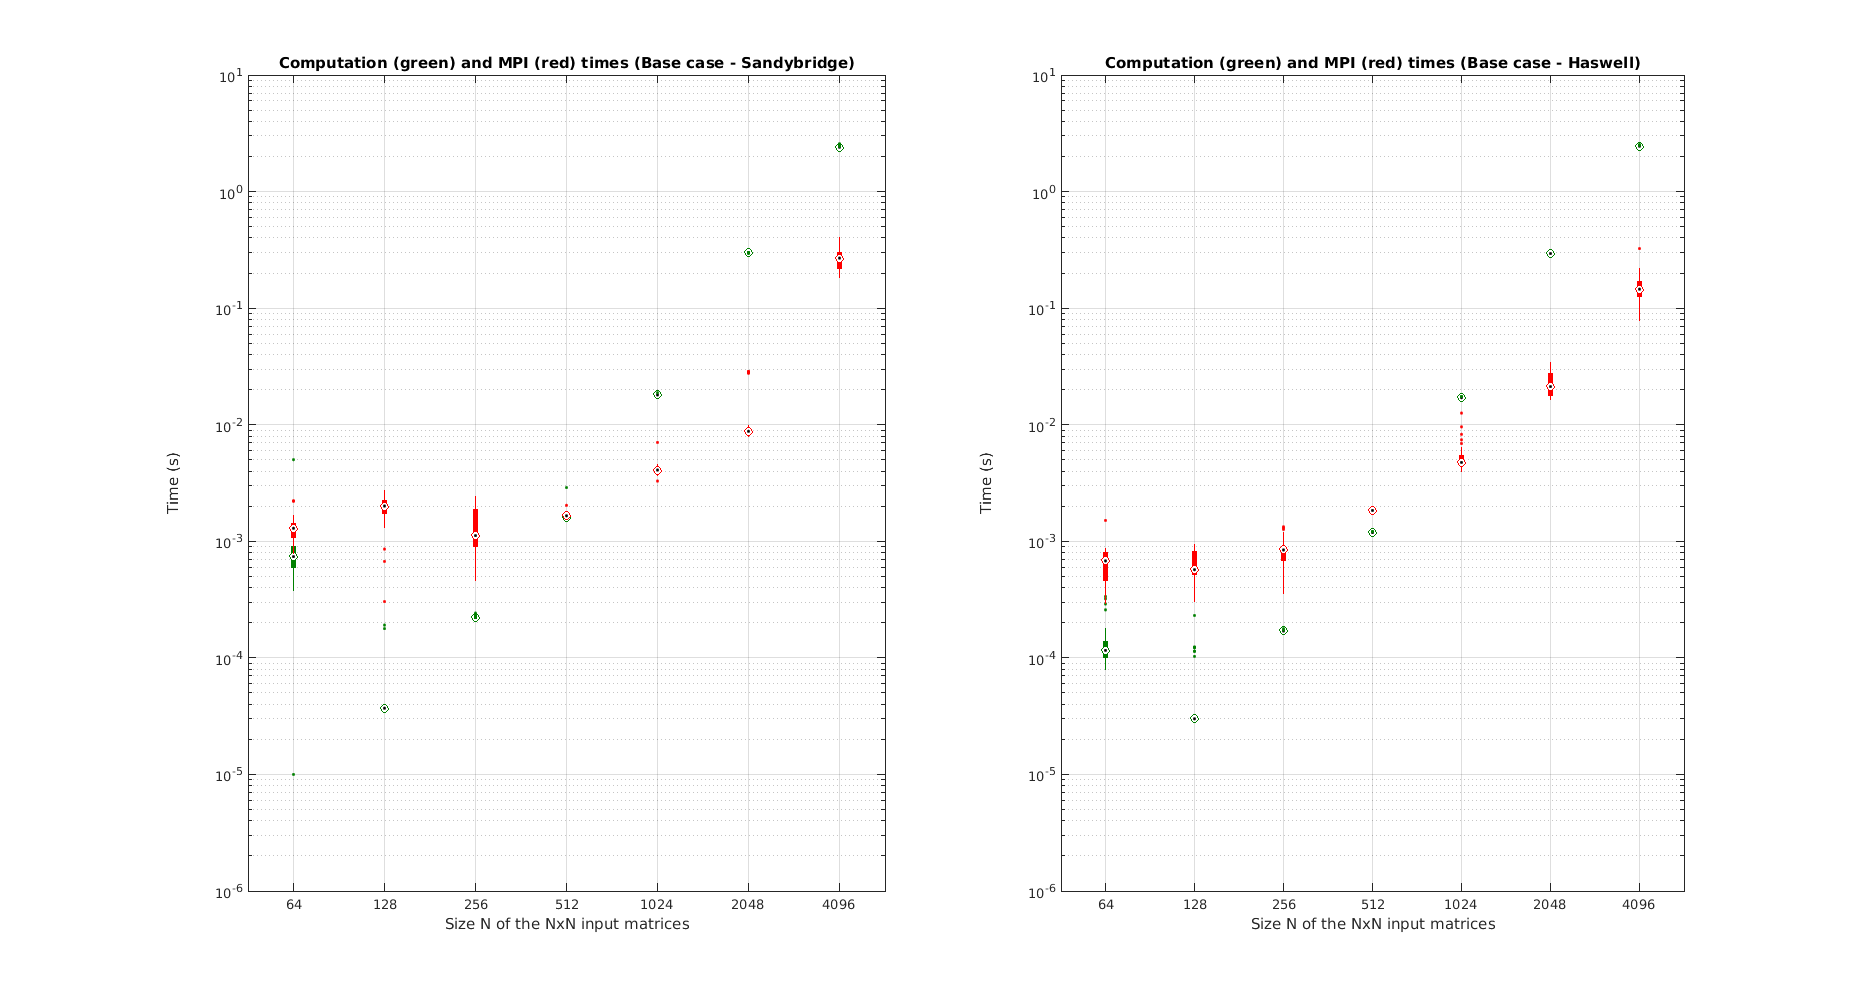
\includegraphics[width=1.1\textwidth]{images/times_provided.png}}
  \caption{Compute time (green) and communication time (red) of Rank0 for Sandybridge (left) and Haswell (right). The points are medians. 30 iterations.}
  \label{fig:times_provided}
  \end{figure}
\end{frame}

\begin{frame}
  \frametitle{Scalability (Base case)}
  \begin{itemize}
  \item N=512 divides each plot to a communication-bounded area (left) and a computation-bounded (right).
  \item Higher variance in smaller sizes.
  \item Almost constant communication time for N < 512.
  \item Computation time increases logarithmically. Higher for N=64.
  \item Haswell performs a bit better in communication. Faster network, higher memory bandwidth, bigger caches. Compiled only with the default optimization (no flags).
  \item Non-blocking tree network topology - maybe we could see some extra variance because of different allocation of the nodes if we had data from multiple job submissions. We can still see clear tendencies with our approach though.
  \end{itemize}
\end{frame}

\begin{frame}
  \frametitle{Tracing with Score-P and Vampir (Base case)}
    \begin{figure}
  \centering
  \makebox[\textwidth][c]{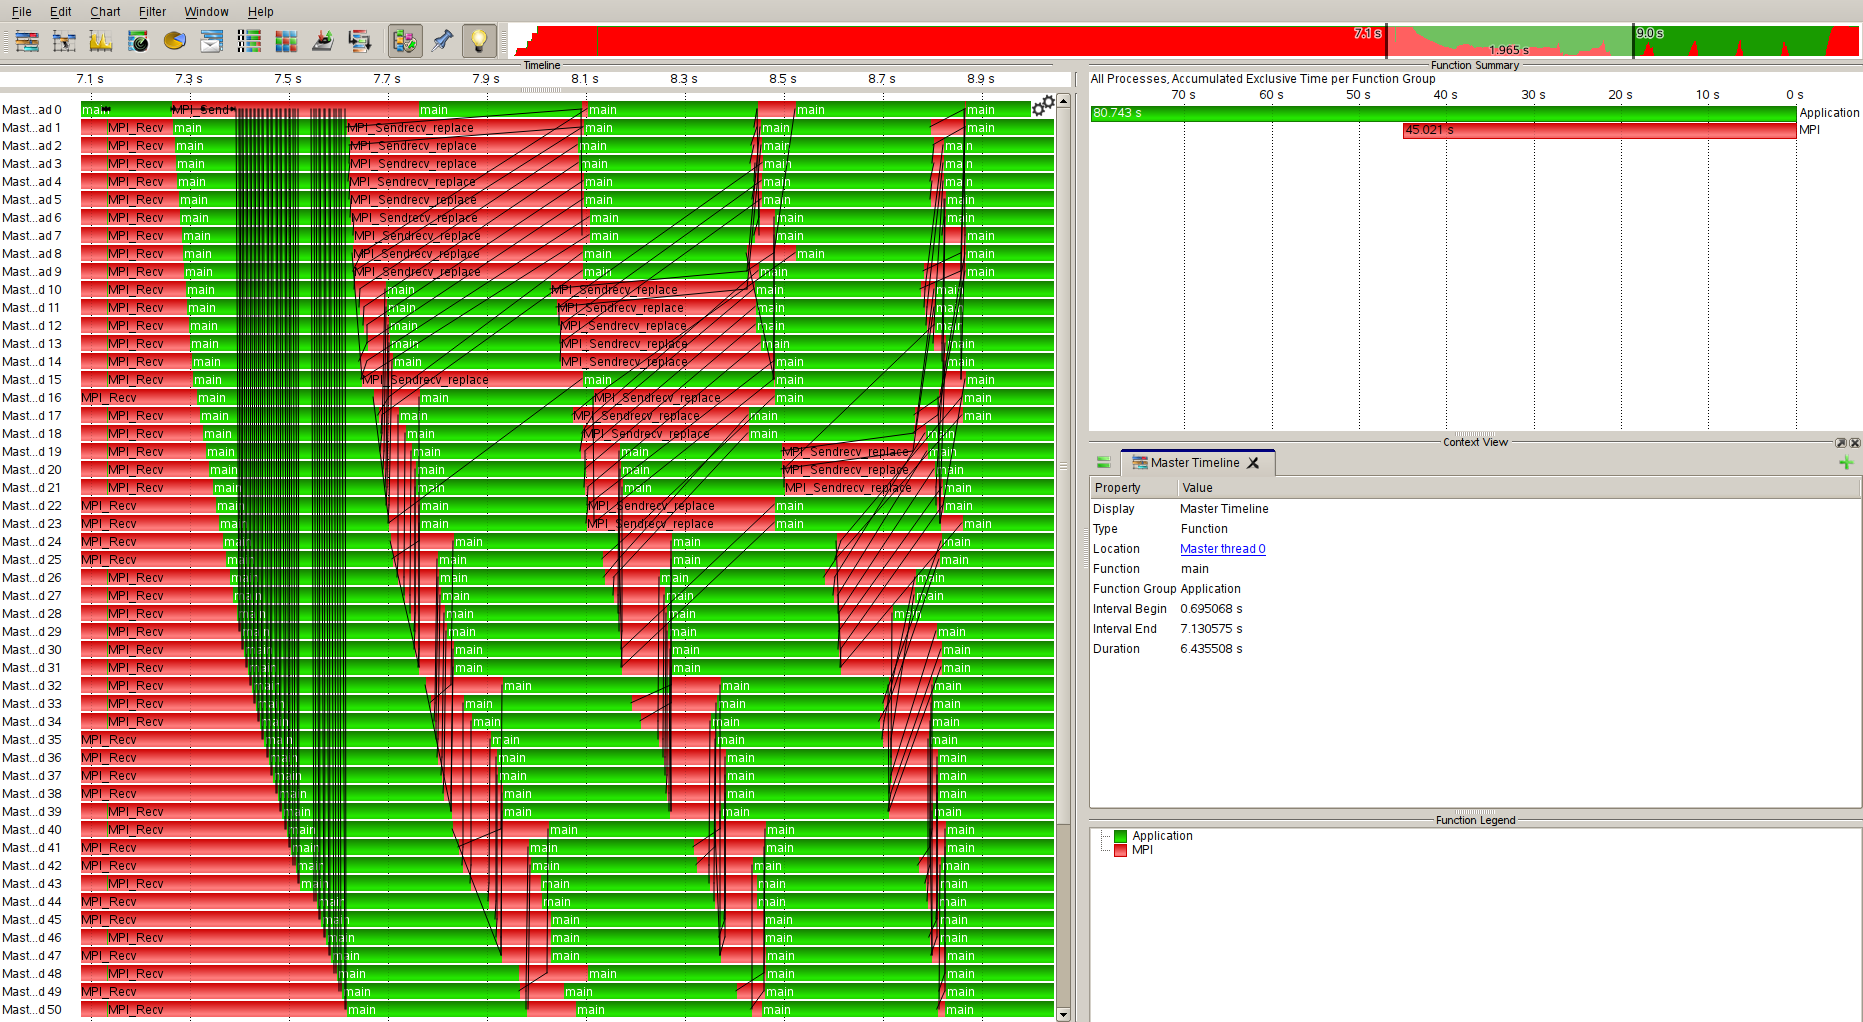
\includegraphics[width=\textwidth]{images/vampir_provided_hw_4096_begin.png}}
  \caption{Tracing for the base case, N=4096, Haswell. Note the peaks of communication activity and the synchronization between senders-receivers.}
  \label{fig:vampir_provided}
  \end{figure}
\end{frame}


\section{Task 4: Non-blocking P2P}
\begin{frame}
  \frametitle{Approach}
  We aim to overlap communication with computation in the main loop. For this, we drop the \texttt{MPI\_Sendrecv()} calls and we use a combination of \texttt{MPI\_Isend()}, \texttt{MPI\_IRecv()}, \texttt{MPI\_Test()} and \texttt{MPI\_Wait()} calls instead.
  
  \begin{itemize}
  \item Goal: Post Send and Receive requests as early as possible. We test the previous communication for completion (buffer re-usage). We wait only if absolutely necessary.
  \item We use another pair of pointers as receive buffers. As soon as we receive, we copy their contents to the local blocks and re-post receive requests immediately.
  \item We try to receive whichever of the A, B blocks is first available.
  \item Several attempts to send:
  \begin{itemize}
  \item As soon as the buffer copy is complete.
  \item In every iteration of the outer loop of the actual computations.
  \item If everything fails, wait and send after the loop.
  \end{itemize}
  \item First and last cycles peeled-off in order to better manage requests and minimize branches.
  \end{itemize}

\end{frame}

\begin{frame}
  \frametitle{Scalability (Nonblocking P2P)}
  \begin{figure}
  \centering
  \makebox[\textwidth][c]{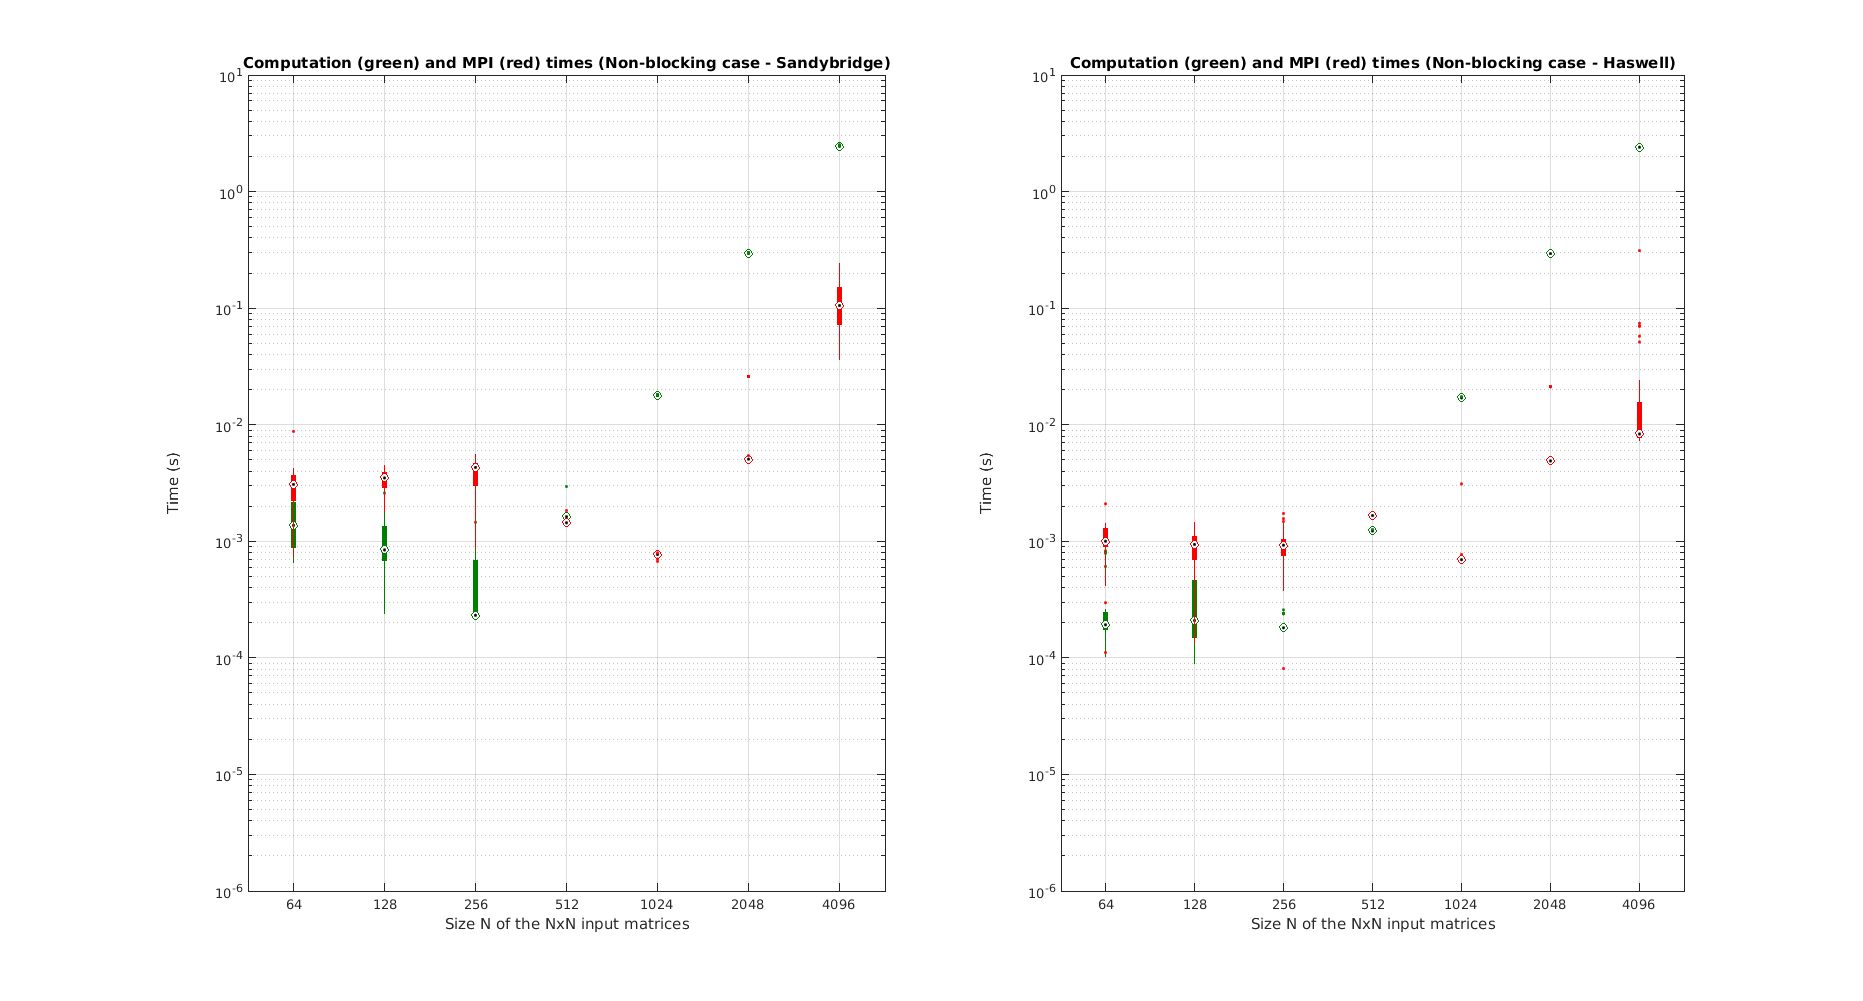
\includegraphics[width=1.1\textwidth]{images/times_nonblocking.png}}
  \caption{Compute time (green) and communication time (red) of Rank0 for Sandybridge (left) and Haswell (right). The points are medians. 30 iterations.}
  \label{fig:times_nonblocking}
  \end{figure}
\end{frame}

\begin{frame}
  \frametitle{Scalability (Nonblocking P2P)}
  \begin{figure}
  \centering
  \makebox[\textwidth][c]{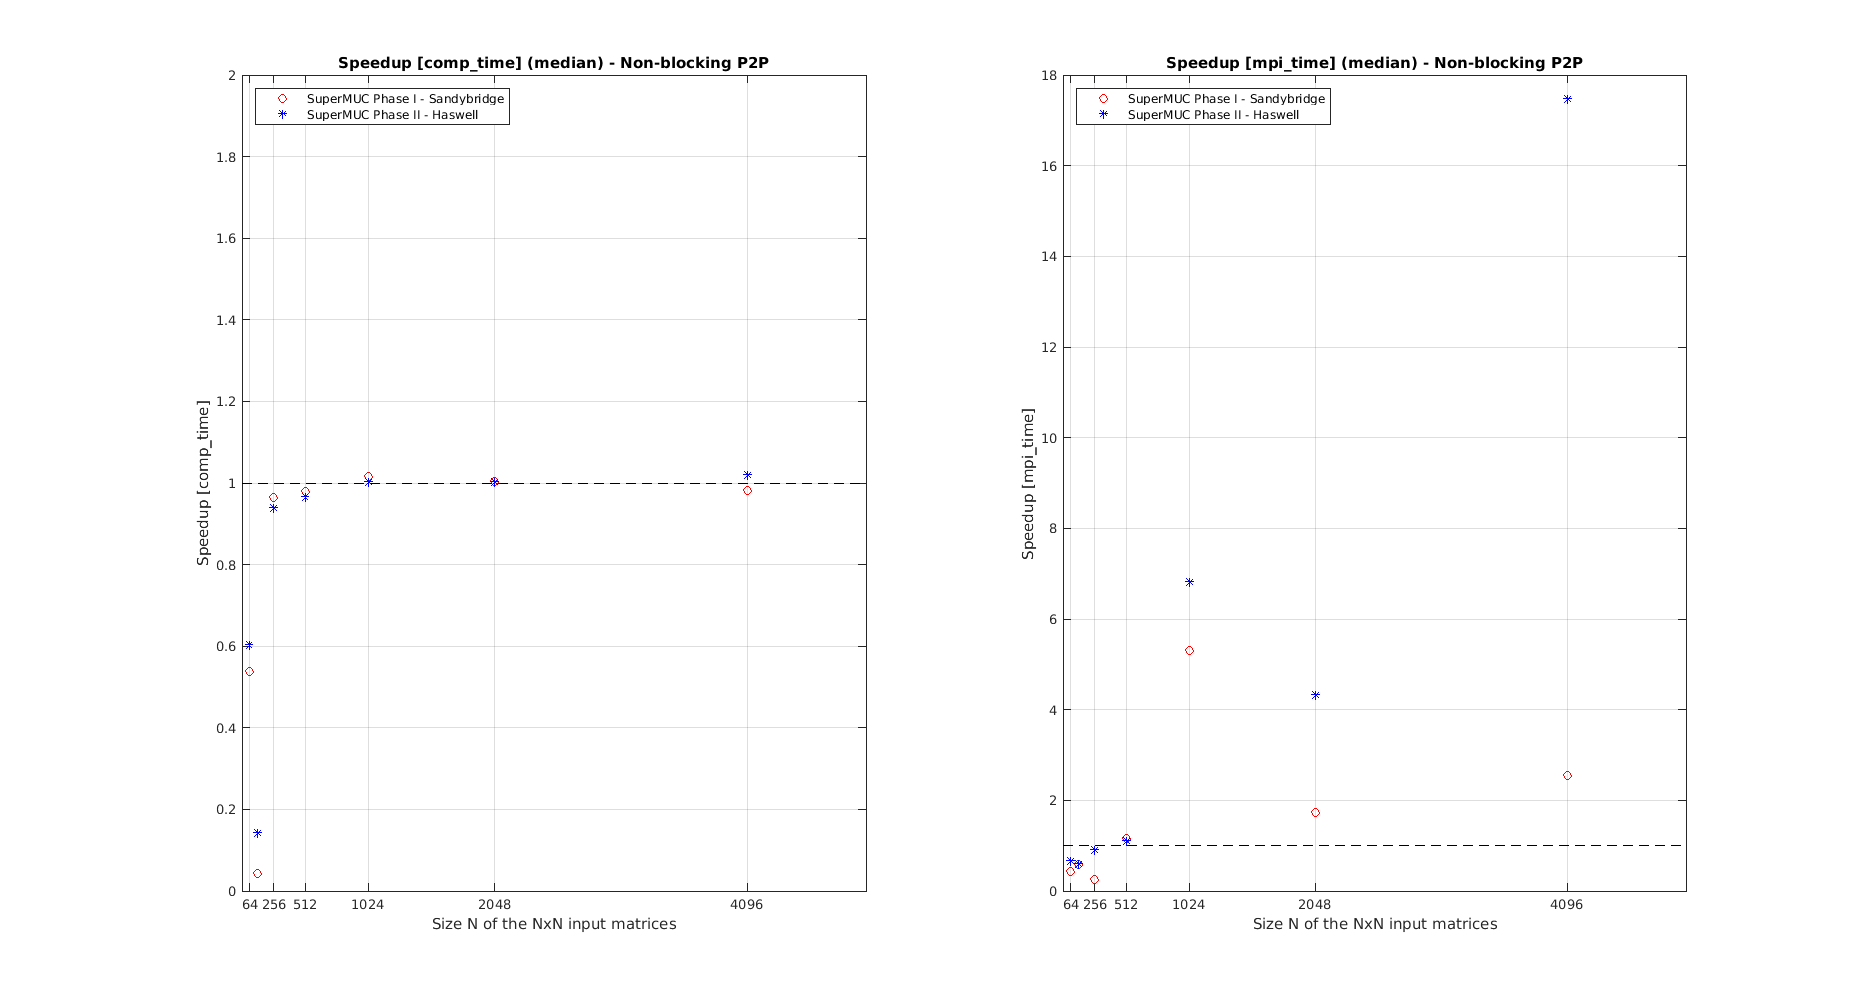
\includegraphics[width=1.1\textwidth]{images/speedup_nonblocking.png}}
  \caption{Speedup with respect to compute time (left) and communication time (right) of Rank0 for Sandybridge (circles) and Haswell (stars). Speedup computed using the medians of 30 iterations.}
  \label{fig:speedup_nonblocking}
  \end{figure}
\end{frame}

\begin{frame}
  \frametitle{Scalability (Nonblocking P2P)}
  \begin{itemize}
  \item Critical point still at N=512.
  \item This communication scheme helps much for larger N but gives worse results at small N.
  \item Similar general behavior in large N as in base case. A bit different in small.
  \item Computation time increases logarithmically. Higher for N=64 and N=128.
  \item This scheme favors the faster network of SuperMUC Phase II.
  \end{itemize}
\end{frame}

\begin{frame}
  \frametitle{Potential to overlap}
  In the base case (e.g. for N=4096), the region of interest is from approximately 8s to 11s. In this, the accumulated exclusive time spent in the application is ~166.6s and in the MPI calls ~28.7s (including some communication out of the loop). 
   
  Using these data, we estimate that communication in the loop takes at most 14\% of the accumulated time. In a perfect overlap, i.e. with zero communication time, we could gain up to 14\% in this region.
  \begin{figure}
  \centering
  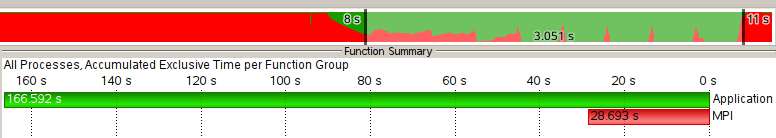
\includegraphics[width=\textwidth]{images/overlap.png}
  \caption{Application and communication time in the region of interest - base case, N=4096, Haswell.}
  \label{fig:overlap_base}
  \end{figure}
\end{frame}

\begin{frame}
  \frametitle{Tracing with Score-P and Vampir (Nonblocking P2P)}
  \begin{figure}
  \centering
  \makebox[\textwidth][c]{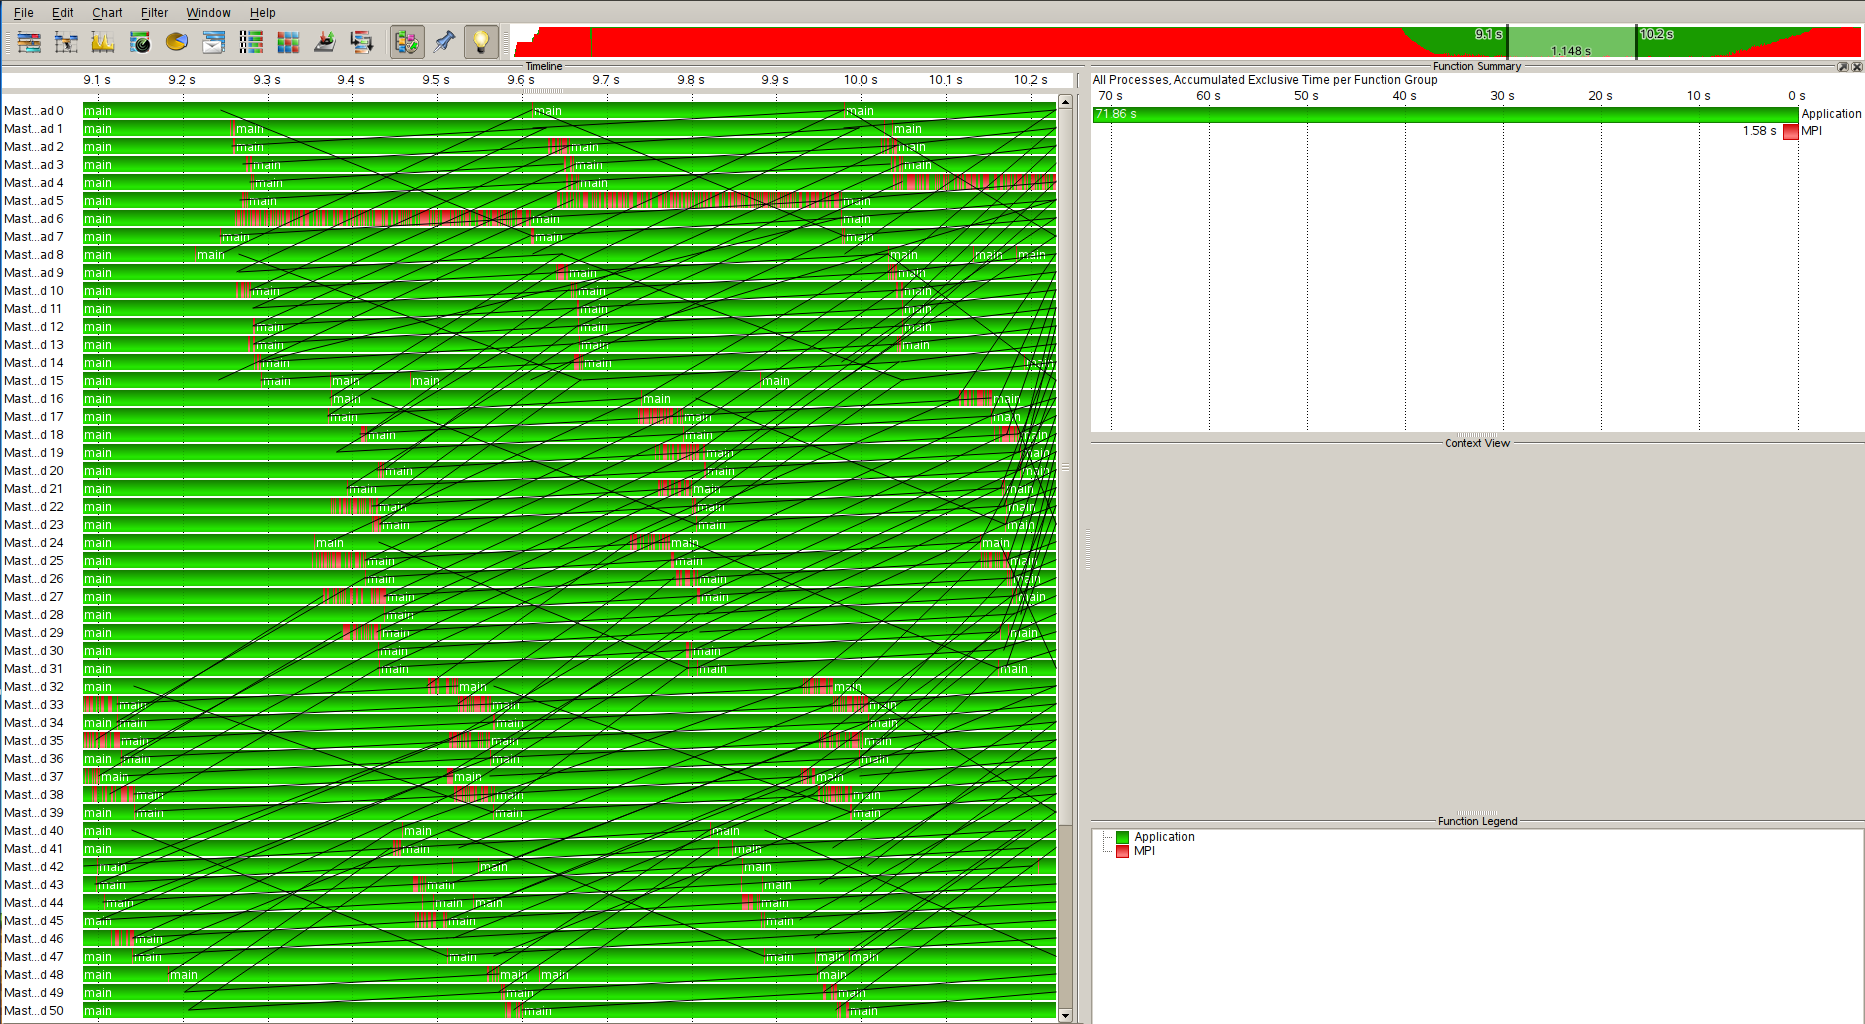
\includegraphics[width=\textwidth]{images/vampir_nonblocking_hw_4096_middle.png}}
  \caption{Tracing for the nonblocking P2P case, N=4096, Haswell. Much better communication-computation overlap is achieved.}
  \label{fig:vampir_nonblocking}
  \end{figure}
\end{frame}

\begin{frame}
  \frametitle{Overlap achieved (Nonblocking P2P)}
  In the non-blocking P2P case we see that, in an inner part of the the region of interest, the communication time corresponds only to approximately to 2\% of the total accumulated time. In other words, the 98\% of the time is used for useful work.
  \begin{figure}
  \centering
  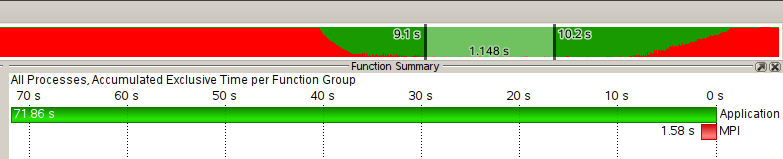
\includegraphics[width=\textwidth]{images/overlap_nonblocking.png}
  \caption{Application and communication time in the region of interest - nonblocking P2P case, N=4096, Haswell.}
  \label{fig:overlap_nonblocking}
  \end{figure}
\end{frame}


\section{Task 5: One-sided communication}
\begin{frame}
  \frametitle{Approach (1)}
  Our initial (and simpler) approach was:
  \begin{itemize}
  \item Create one window for each of A,B that point to the (new) pointers \texttt{A\_shared\_block} and \texttt{B\_shared\_block}. They are used in the same way as the receive buffers in the nonblocking case.
  \item Synchronize the windows with \texttt{MPI\_Win\_fence()}.
  \item Copy the shared blocks to the local blocks.
  \item Synchronize the windows again.
  \item Put the local blocks to the shared blocks of the neighbors using \texttt{MPI\_Put()}.
  \item Perform the actual computations with the local blocks.
  \end{itemize}
\end{frame}

\begin{frame}
  \frametitle{Approach (2)}
  Trying to improve the overlap, we extended our initial approach to use two windows, alternately. The idea is to fence the individual windows less frequently, in order to allow more time for communication completion.

  For this, we create two windows for each matrix, that each corresponds to another pointer. After filling both pointers, the second one is always one step ahead than the first.
  
  Again, we peel-off the first and last cycles, in order to better balance the communication operations without adding even more branches. Inside the loop, we use the loop index to swap between the windows.
\end{frame}

\begin{frame}
  \frametitle{Scalability (One-sided)}
  \begin{figure}
  \centering
  \makebox[\textwidth][c]{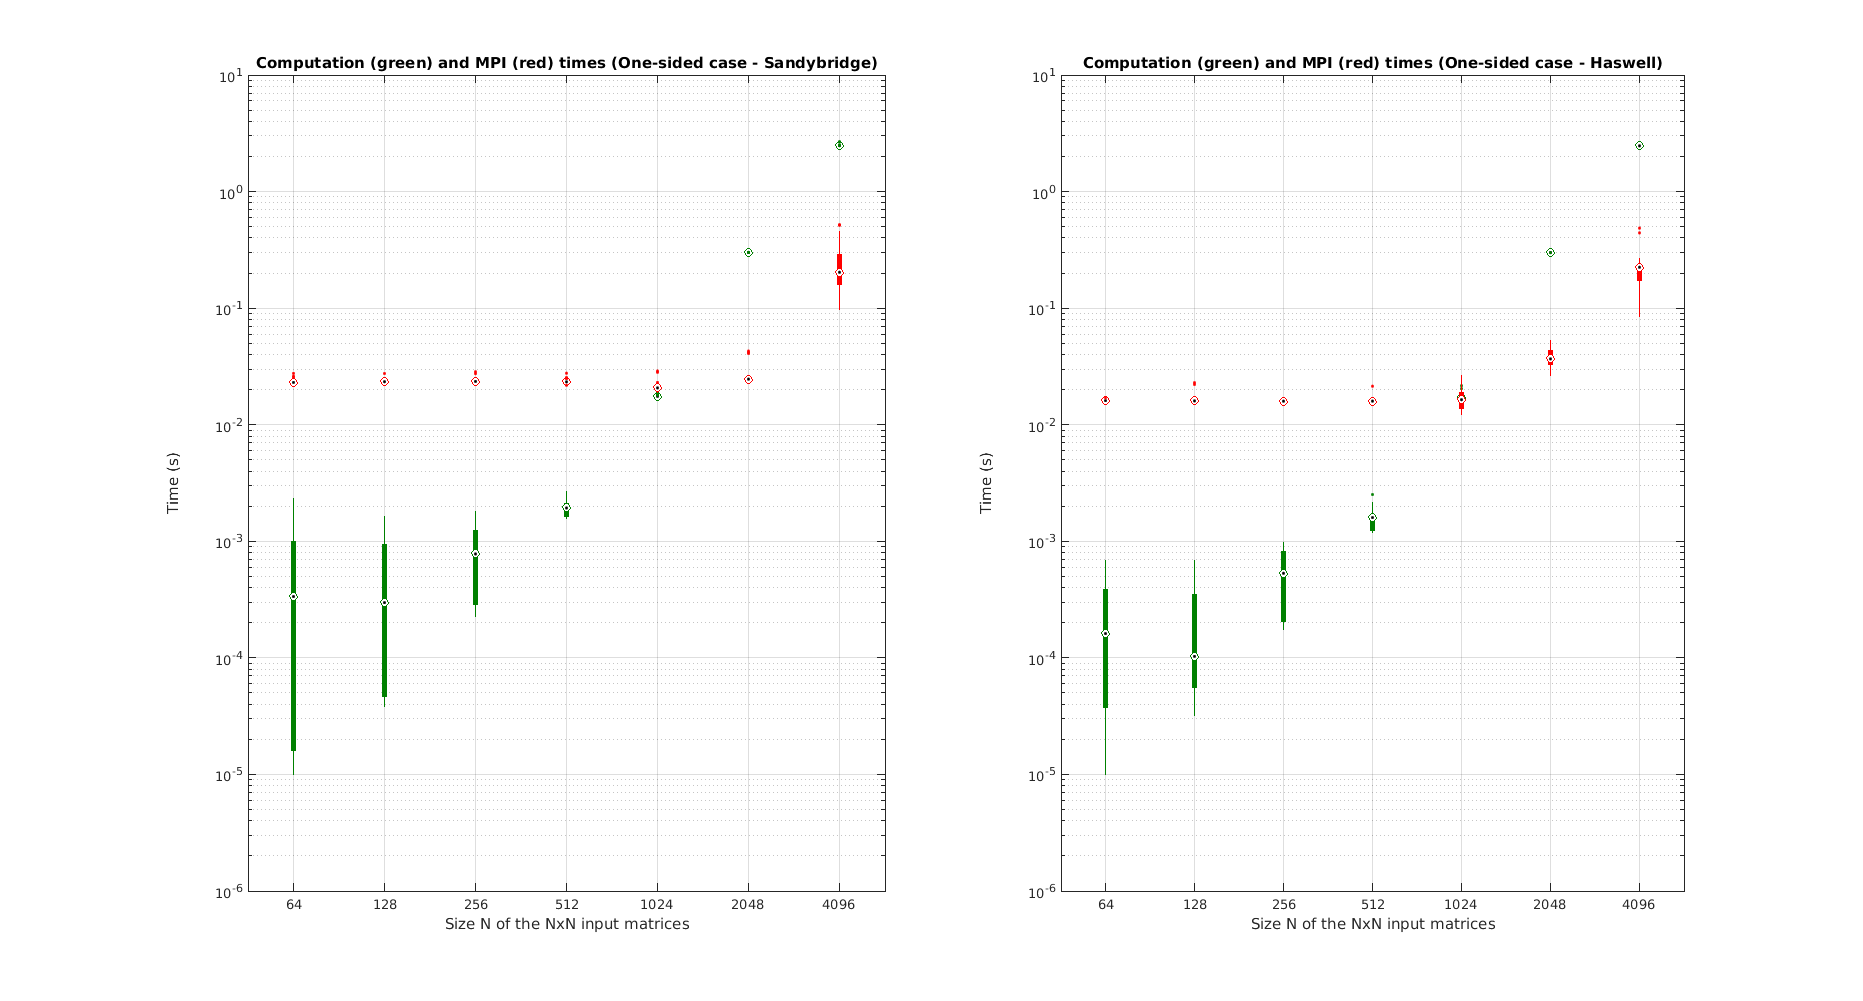
\includegraphics[width=1.1\textwidth]{images/times_onesided.png}}
  \caption{Compute time (green) and communication time (red) of Rank0 for Sandybridge (left) and Haswell (right). The points are medians. 30 iterations.}
  \label{fig:times_onesided}
  \end{figure}
\end{frame}

\begin{frame}
  \frametitle{Scalability (One-sided)}
  \begin{figure}
  \centering
  \makebox[\textwidth][c]{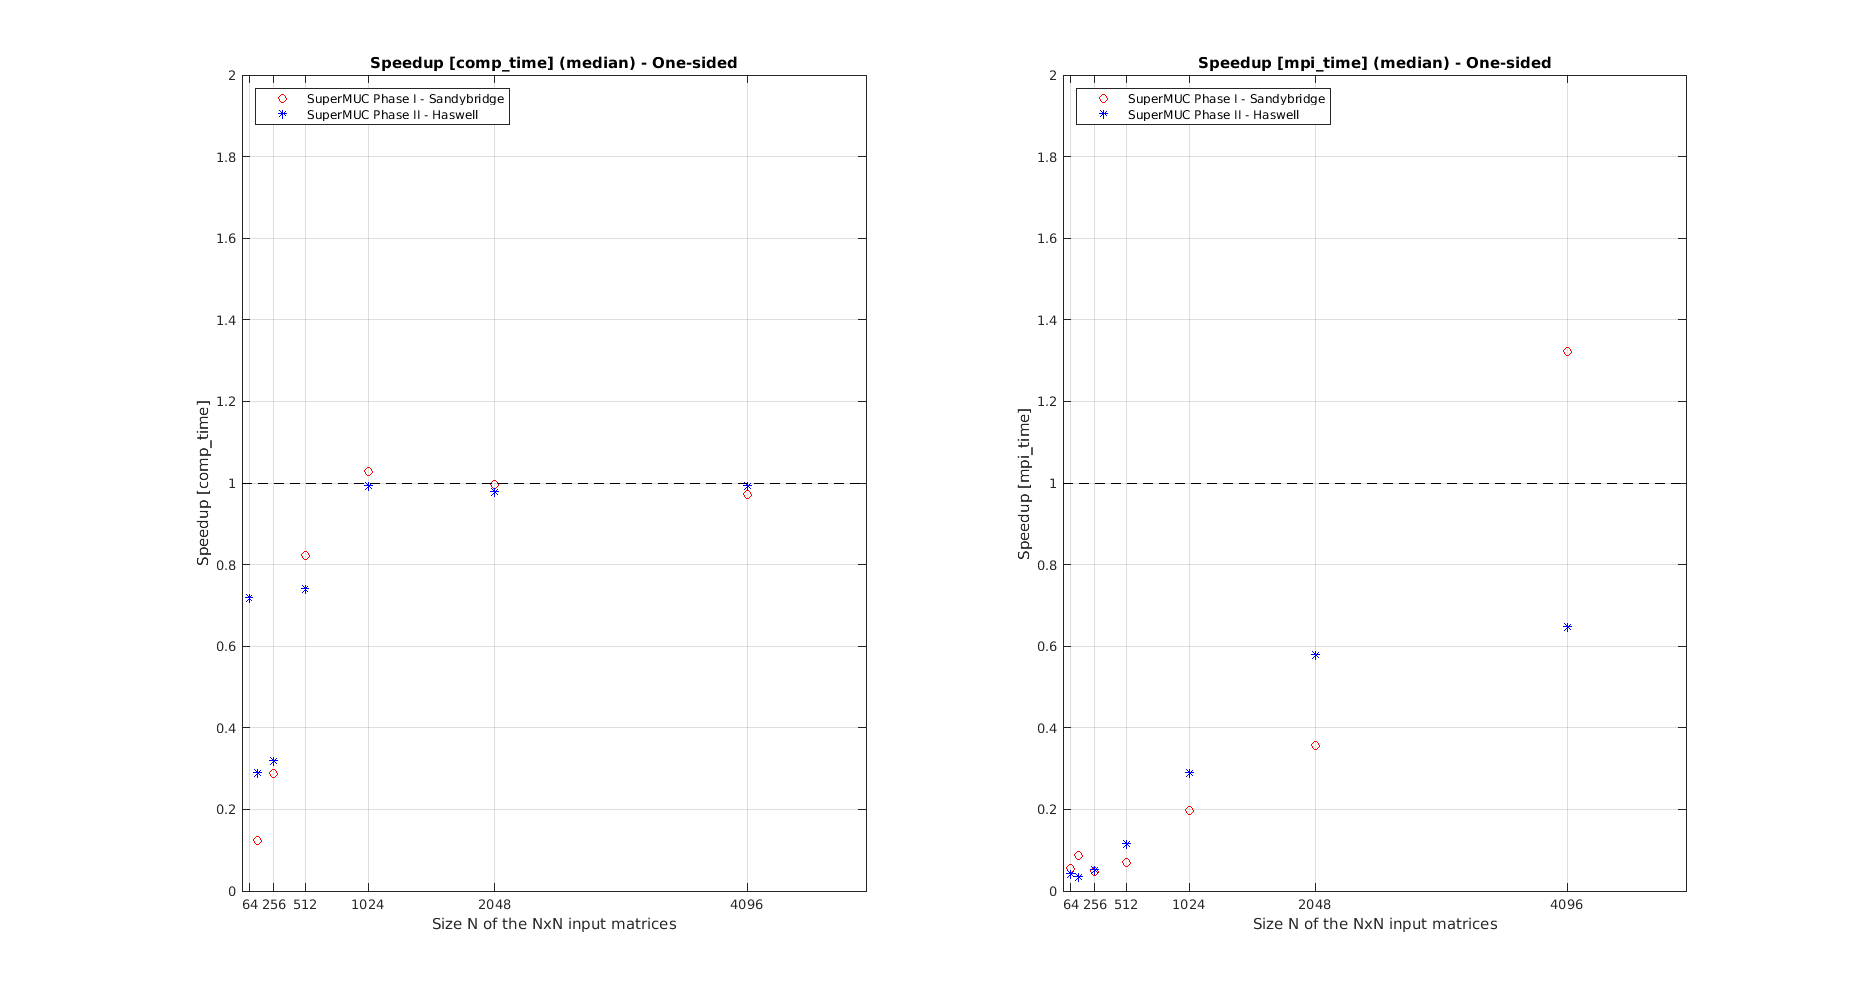
\includegraphics[width=1.1\textwidth]{images/speedup_onesided.png}}
  \caption{Speedup with respect to compute time (left) and communication time (right) of Rank0 for Sandybridge (circles) and Haswell (stars). Speedup computed using the medians of 30 iterations.}
  \label{fig:speedup_onesided}
  \end{figure}
\end{frame}

\begin{frame}
  \frametitle{Scalability (One-sided)}
    \begin{itemize}
    \item Worse results than both the base and the non-blocking case for these problem sizes.
    \item Still, the two-window method performed a bit better than our initial one-window approach.
    \item Significantly longer communication time, almost constant and very reproducible.
    \item Critical point moved at N=1024.
    \item Much worse for small N, unkown behavior above N=4096.
    \item Large variance in computation time below N=1024. Maybe energy management? Again reproducible in the compute-bounded area.
    \item In the most cases, Haswell performs better.
  \end{itemize}
\end{frame}

\begin{frame}
  \frametitle{Tracing with Score-P and Vampir (One-sided)}
  \begin{figure}
  \centering
  \makebox[\textwidth][c]{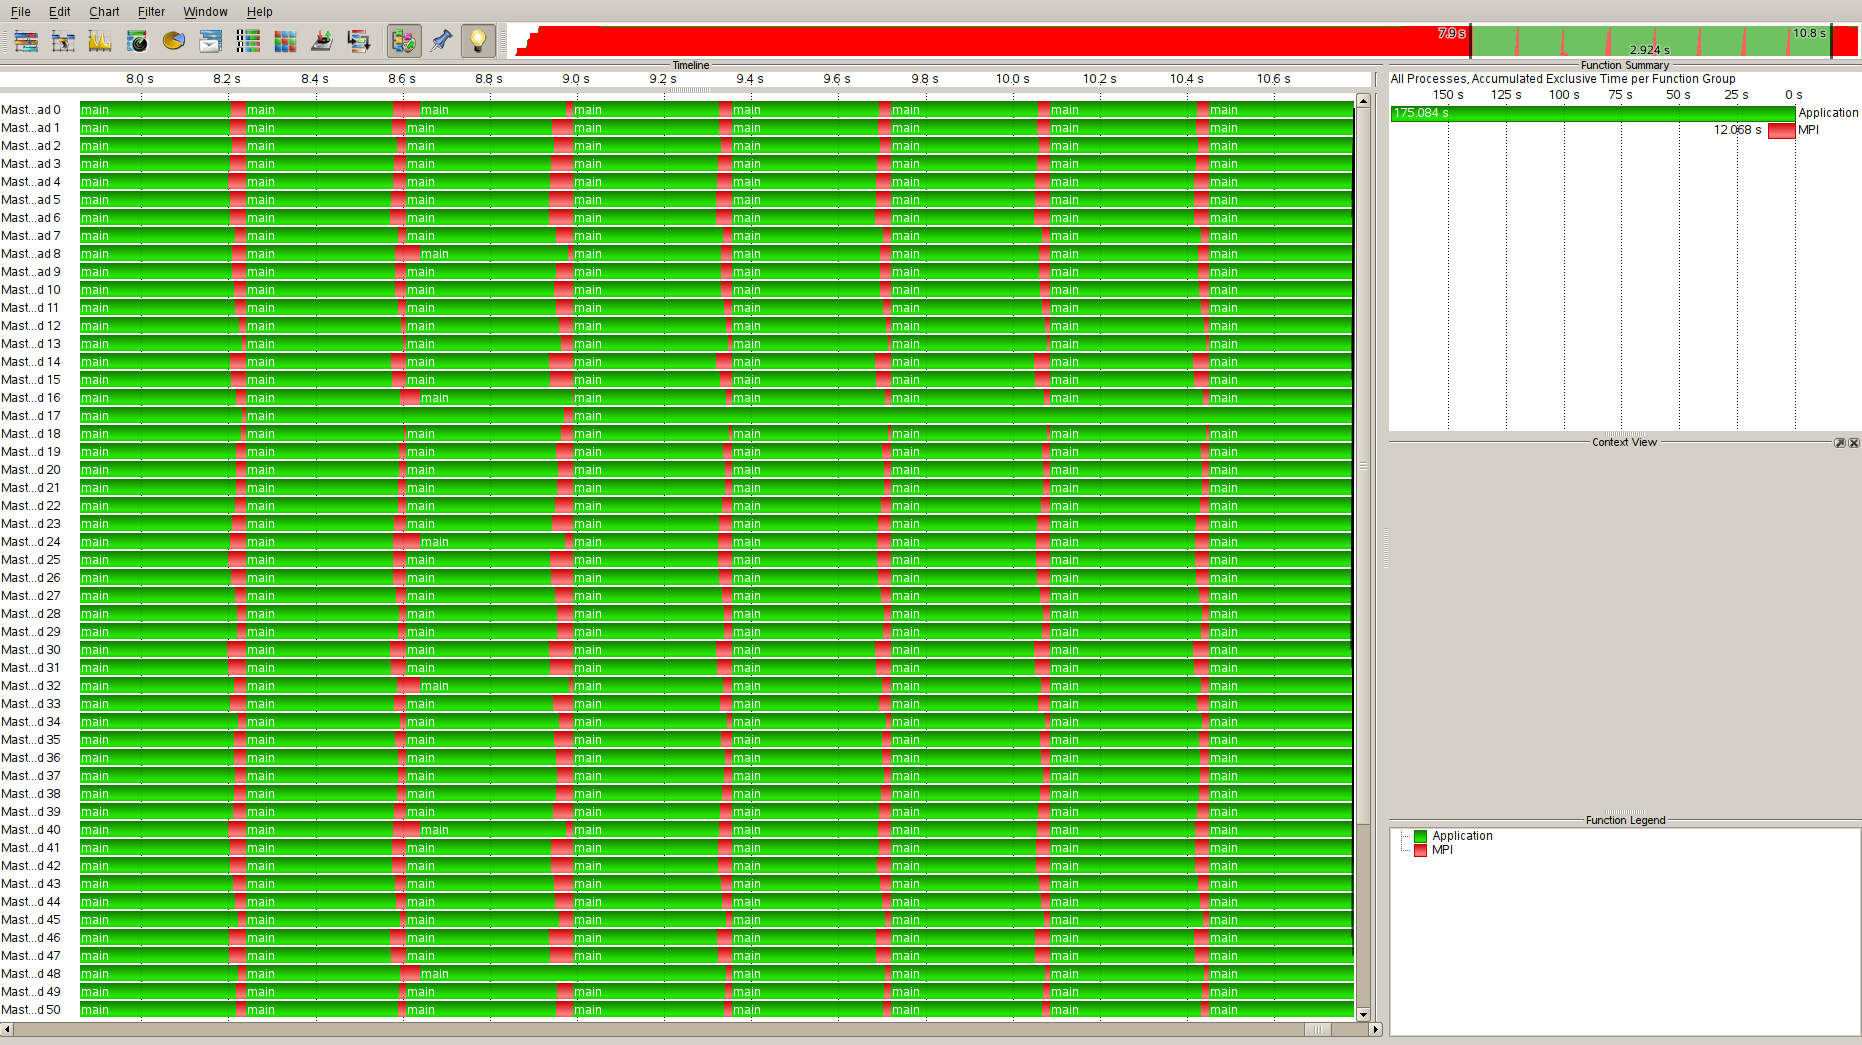
\includegraphics[width=\textwidth]{images/vampir_onesided_hw_4096_middle.png}}
  \caption{Tracing for the one-sided case, N=4096, Haswell.}
  \label{fig:vampir_onesided}
  \end{figure}
\end{frame}

\begin{frame}
  \frametitle{Overlap achieved (One-sided)}
  In the one-sided case we observe that, it the region of interest (that is here easier to define), the communication time corresponds to the 6\% of the overall accumulated time. Not as good as in the non-blocking case, but better than the base case. 
  
  Please note that in our implementation we include in the \texttt{mpi\_time} also non-mpi regions that we added because of our approach to the communication scheme. 
  \begin{figure}
  \centering
  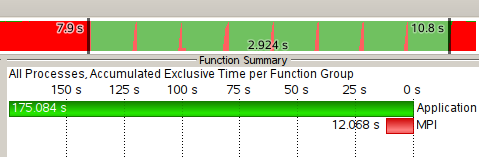
\includegraphics[width=0.8\textwidth]{images/overlap_onesided.png}
  \caption{Application and communication time in the region of interest - nonblocking P2P case, N=4096, Haswell.}
  \label{fig:overlap_onesided}
  \end{figure}
\end{frame}

\section{Conclusions}
\begin{frame}
  \frametitle{Conclusions}
  \begin{itemize}
      \item There is some optimization potential for the provided Cannon's algorithm implementation.
      \item The application is communication-bounded under N=512 or N=1024 and compute-bounded above.
      \item Non-blocking P2P communication achieves good overlap and helps more in the case of SuperMUC Phase II.
      \item Our one-sided communication did not turn to improve the performance according neither to the non-blocking or the base case. But there seems to be a tendency to help in bigger problems.
      \item SuperMUC Phase II seems to perform generally better for this application.
      \item Tracing proved to be very useful during our investigations.
  \end{itemize}
\end{frame}

\section{Future work}
\begin{frame}
  \frametitle{Future work}
  To improve the performance of this application more, one could try:
  \begin{itemize}
  \item Implement a parallel input scheme, to reduce the initial overhead.
  \item Change the blocking communication between Rank0 and the rest of the processes with non-blocking P2P or collectives.
  \item Investigate the scaling up to bigger matrix sizes, especially for the one-sided communication.
  \item Investigate the effect of compiler optimizations.
  \end{itemize}

\end{frame}

\end{document}
